\documentclass[a4paper, 14pt]{extarticle}
\usepackage{float}
% Поля
%--------------------------------------
\usepackage{geometry}
\geometry{a4paper,tmargin=2cm,bmargin=2cm,lmargin=3cm,rmargin=1cm}
%--------------------------------------


%Russian-specific packages
%--------------------------------------
\usepackage[T2A]{fontenc}
\usepackage[utf8]{inputenc}
\usepackage[english, main=russian]{babel}
%--------------------------------------

\usepackage{textcomp}

% Красная строка
%--------------------------------------
\usepackage{indentfirst}
%--------------------------------------


%Graphics
%--------------------------------------
\usepackage{graphicx}
\graphicspath{ {./images/} }
\usepackage{wrapfig}
%--------------------------------------

% Полуторный интервал
%--------------------------------------
\linespread{1.3}
%--------------------------------------

%Выравнивание и переносы
%--------------------------------------
% Избавляемся от переполнений
\sloppy
% Запрещаем разрыв страницы после первой строки абзаца
\clubpenalty=10000
% Запрещаем разрыв страницы после последней строки абзаца
\widowpenalty=10000
%--------------------------------------

%Списки
\usepackage{enumitem}

%Подписи
\usepackage{caption}

%Гиперссылки
\usepackage{hyperref}

\usepackage{float}

\hypersetup {
	unicode=true
}

%Рисунки
%--------------------------------------
\DeclareCaptionLabelSeparator*{emdash}{~--- }
\captionsetup[figure]{labelsep=emdash,font=onehalfspacing,position=bottom}
%--------------------------------------

\usepackage{tempora}

%Листинги
%--------------------------------------
\usepackage{listings}
\lstset{
  basicstyle=\ttfamily\footnotesize,
  %basicstyle=\footnotesize\AnkaCoder,        % the size of the fonts that are used for the code
  breakatwhitespace=false,        % sets if automatic breaks shoulbd only happen at whitespace
  breaklines=true,                 % sets automatic line breaking
  captionpos=t,                    % sets the caption-position to bottom
  inputencoding=utf8,
  frame=single,                    % adds a frame around the code
  keepspaces=true,                 % keeps spaces in text, useful for keeping indentation of code (possibly needs columns=flexible)
  keywordstyle=\bf,       % keyword style
  numbers=left,                    % where to put the line-numbers; possible values are (none, left, right)
  numbersep=5pt,                   % how far the line-numbers are from the code
  xleftmargin=25pt,
  xrightmargin=25pt,
  showspaces=false,                % show spaces everywhere adding particular underscores; it overrides 'showstringspaces'
  showstringspaces=false,          % underline spaces within strings only
  showtabs=false,                  % show tabs within strings adding particular underscores
  stepnumber=1,                    % the step between two line-numbers. If it's 1, each line will be numbered
  tabsize=2,                       % sets default tabsize to 8 spaces
  title=\lstname                   % show the filename of files included with \lstinputlisting; also try caption instead of title
}
%--------------------------------------

%%% Математические пакеты %%%
%--------------------------------------
\usepackage{amsthm,amsfonts,amsmath,amssymb,amscd}  % Математические дополнения от AMS
\usepackage{mathtools}                              % Добавляет окружение multlined
\usepackage[perpage]{footmisc}
%--------------------------------------

%--------------------------------------
%			НАЧАЛО ДОКУМЕНТА
%--------------------------------------

\begin{document}

%--------------------------------------
%			ТИТУЛЬНЫЙ ЛИСТ
%--------------------------------------
\begin{titlepage}
\thispagestyle{empty}
\newpage


%Шапка титульного листа
%--------------------------------------
\vspace*{-60pt}
\hspace{-65pt}
\begin{minipage}{0.3\textwidth}
\hspace*{-20pt}\centering

\includegraphics[width=\textwidth]{emblem}
\end{minipage}
\begin{minipage}{0.67\textwidth}\small \textbf{
\vspace*{-0.7ex}
\hspace*{-6pt}\centerline{Министерство науки и высшего образования Российской Федерации}
\vspace*{-0.7ex}
\centerline{Федеральное государственное бюджетное образовательное учреждение }
\vspace*{-0.7ex}
\centerline{высшего образования}
\vspace*{-0.7ex}
\centerline{<<Московский государственный технический университет}
\vspace*{-0.7ex}
\centerline{имени Н.Э. Баумана}
\vspace*{-0.7ex}
\centerline{(национальный исследовательский университет)>>}
\vspace*{-0.7ex}
\centerline{(МГТУ им. Н.Э. Баумана)}}
\end{minipage}
%--------------------------------------

%Полосы
%--------------------------------------
\vspace{-25pt}
\hspace{-35pt}\rule{\textwidth}{2.3pt}

\vspace*{-20.3pt}
\hspace{-35pt}\rule{\textwidth}{0.4pt}
%--------------------------------------

\vspace{1.5ex}
\hspace{-35pt} \noindent \small ФАКУЛЬТЕТ\hspace{80pt} <<Информатика и системы управления>>

\vspace*{-16pt}
\hspace{47pt}\rule{0.83\textwidth}{0.4pt}

\vspace{0.5ex}
\hspace{-35pt} \noindent \small КАФЕДРА\hspace{50pt} <<Теоретическая информатика и компьютерные технологии>>

\vspace*{-16pt}
\hspace{30pt}\rule{0.866\textwidth}{0.4pt}

\vspace{11em}

\begin{center}
\Large {\bf Лабораторная работа № 5} \\
\large {\bf по курсу <<Теория искусственных нейронных сетей>>} \\
\large <<Сверточные нейронные сети>>
\end{center}\normalsize

\vspace{8em}


\begin{flushright}
  {Студент группы ИУ9-71Б Баев Д.А \hspace*{15pt}\\
  \vspace{2ex}
  Преподаватель Каганов Ю. Т.\hspace*{15pt}}
\end{flushright}

\bigskip

\vfill


\begin{center}
\textsl{Москва 2023}
\end{center}
\end{titlepage}
%--------------------------------------
%		КОНЕЦ ТИТУЛЬНОГО ЛИСТА
%--------------------------------------

\renewcommand{\ttdefault}{pcr}

\setlength{\tabcolsep}{3pt}
\newpage
\setcounter{page}{2}

\section{Задание}\label{Sect::task}
1. LeNet.

2. VGG.

3. ResNet.

4. Подготовить отчет с распечаткой текста программы, графиками
результатов исследования и анализом результатов.
\newpage
\section{Исходный код}

Исходный код программы представлен в листингах~\ref{lst:code1}-~\ref{lst:code5}

\begin{lstlisting}[language={},caption={Подготовка датасета},label={lst:code1}, breaklines=true]
from torch import nn
from tqdm import tqdm

from torchvision.datasets import mnist, cifar
from torchvision import transforms

from torch.utils.data import DataLoader, Subset
import matplotlib.pyplot as plt
import torch

device = 'cuda' if torch.cuda.is_available() else 'cpu'
device

batch_size = 8
batches_per_epoch = 128
test_size_mnist = 128
train_size_mnist = 5120
test_size_cifar = 1024
train_size_cifar = 48976

mnist_dataset = mnist.MNIST(
    root = 'data',
    train=True,
    download=True,
    transform=transforms.ToTensor()
)

mnist_dataloader = {
    "train": DataLoader(Subset(mnist_dataset, range(test_size_mnist, test_size_mnist + train_size_mnist)), shuffle=True, batch_size=batch_size),
    "test": DataLoader(Subset(mnist_dataset, range(0, test_size_mnist)), shuffle=True, batch_size=batch_size)
}

transform = transforms.Compose([
    transforms.RandomCrop(32, padding=4),
    transforms.RandomHorizontalFlip(),
    transforms.ToTensor(),
    transforms.Normalize((0.4914, 0.4822, 0.4465), (0.2023, 0.1994, 0.2010))
])

cifar_dataset = cifar.CIFAR10(
    root='data',
    train=True,
    download=True,
    transform=transform
)

cifar_dataloader = {
    "train": DataLoader(Subset(cifar_dataset, range(test_size_cifar, test_size_cifar + train_size_cifar)), shuffle=True, batch_size=batch_size),
    "test": DataLoader(Subset(cifar_dataset, range(0, test_size_cifar)), shuffle=True, batch_size=batch_size)
}
\end{lstlisting}


\begin{lstlisting}[language={},caption={LeNet},label={lst:code2}, breaklines=true]
class LeNet(nn.Module):
    def __init__(self):
        super(LeNet, self).__init__()

        self.conv = nn.Sequential(
            nn.Conv2d(in_channels=1, out_channels=6, kernel_size=5, padding=2),
            nn.ReLU(),
            nn.MaxPool2d(kernel_size=2, stride=2),
            nn.Conv2d(in_channels=6, out_channels=16, kernel_size=5),
            nn.ReLU(),
            nn.MaxPool2d(kernel_size=2, stride=2)
        )

        self.fc = nn.Sequential(
            nn.Linear(in_features=16*5*5, out_features=120),
            nn.ReLU(),
            nn.Linear(in_features=120, out_features=84),
            nn.ReLU(),
            nn.Linear(in_features=84, out_features=10)
        )

    def forward(self, image):
        output = self.conv(image)
        output = self.fc(output.view(image.shape[0], -1))
        return output
\end{lstlisting}




\begin{lstlisting}[language={},caption={MiniVGG},label={lst:code3}, breaklines=true]
class MiniVGG(nn.Module):
    def __init__(self):
        super(MiniVGG, self).__init__()

        self.features = nn.Sequential(
            nn.Conv2d(3, 64, kernel_size=3, padding=1),
            nn.ReLU(inplace=True),
            nn.Conv2d(64, 64, kernel_size=3, padding=1),
            nn.ReLU(inplace=True),
            nn.MaxPool2d(kernel_size=2, stride=2),

            nn.Conv2d(64, 128, kernel_size=3, padding=1),
            nn.ReLU(inplace=True),
            nn.Conv2d(128, 128, kernel_size=3, padding=1),
            nn.ReLU(inplace=True),
            nn.MaxPool2d(kernel_size=2, stride=2)
        )

        self.classifier = nn.Sequential(
            nn.Linear(128 * 8 * 8, 512),
            nn.ReLU(inplace=True),
            nn.Dropout(),
            nn.Linear(512, 256),
            nn.ReLU(inplace=True),
            nn.Dropout(),
            nn.Linear(256, 10)
        )

    def forward(self, image):
        output = self.features(image)
        output = output.view(image.shape[0], -1)
        output = self.classifier(output)
        return output
\end{lstlisting}


\begin{lstlisting}[language={},caption={ResNet},label={lst:code4}, breaklines=true]
class ResidualBlock(nn.Module):
    def __init__(self, in_ch, out_ch, stride=1):
        super(ResidualBlock, self).__init__()
        self.conv1 = nn.Sequential(
            nn.Conv2d(in_ch, out_ch, kernel_size=3, stride=stride, padding=1),
            nn.BatchNorm2d(out_ch),
            nn.ReLU()
        )
        self.conv2 = nn.Sequential(
            nn.Conv2d(out_ch, out_ch, kernel_size=3, stride=1, padding=1),
            nn.BatchNorm2d(out_ch)
        )
        self.relu = nn.ReLU()
        if in_ch != out_ch:
            self.downsaple = nn.Conv2d(in_ch, out_ch, kernel_size=3, stride=2, padding=1)
        else:
            self.downsaple = None

    def forward(self, image):
        residual = image
        output = self.conv1(image)
        output = self.conv2(output)
        if self.downsaple is not None:
            residual = self.downsaple(residual)
        output += residual
        output = self.relu(output)
        return output

class ResNet(nn.Module):
    def __init__(self):
        super(ResNet, self).__init__()
        self.conv1 = nn.Sequential(
            nn.Conv2d(3, 16, kernel_size=3, stride=1, padding=1),
            nn.BatchNorm2d(16),
            nn.ReLU()
        )
        self.layer1 = ResidualBlock(16, 16, 1)
        self.layer2 = ResidualBlock(16, 32, 2)
        self.layer3 = ResidualBlock(32, 64, 2)
        self.avgpool = nn.AvgPool2d(7, stride=2)
        self.fc = nn.Sequential(
            nn.BatchNorm1d(64),
            nn.Linear(64, 128),
            nn.ReLU(),
            nn.BatchNorm1d(128),
            nn.Linear(128, 10)
        )
    def forward(self, image):
        output = self.conv1(image)
        output = self.layer1(output)
        output = self.layer2(output)
        output = self.layer3(output)
        output = self.avgpool(output)
        output = output.view(image.shape[0], -1)
        output = self.fc(output)
        return output
\end{lstlisting}




\begin{lstlisting}[language={},caption={Обучение модели},label={lst:code5}, breaklines=true]
def train_model_and_plot(model, optimizer, dataloader, epochs=50, lr=0.001):
    model.to(device)
    train_acc, test_acc = [], []
    if optimizer == "NAG":
        optimizer = torch.optim.SGD(model.parameters(), lr=lr, nesterov=True, momentum=0.9)
    else:
        optimizer = optimizer(model.parameters(), lr=lr)
    loss_fn = nn.CrossEntropyLoss()

    for epoch in tqdm(range(epochs)):
        if epoch == 200:
            optimizer.param_groups[0]['lr'] /= 10
        running_accuracy = 0
        i = 0
        for x, y in dataloader["train"]:
            x, y = x.to(device), y.to(device)
            prediction = model(x)
            loss = loss_fn(prediction, y)
            running_accuracy += (prediction.softmax(dim=1).argmax(dim=1) == y).float().mean()
            optimizer.zero_grad()
            loss.backward()
            optimizer.step()
            i += 1
            if i == batches_per_epoch:
                break
        running_accuracy /= batches_per_epoch
        train_acc.append(running_accuracy.cpu())

        with torch.no_grad():
            running_accuracy = 0
            for x, y in dataloader['test']:
                x, y = x.to(device), y.to(device)
                prediction = model(x)
                running_accuracy += (prediction.softmax(dim=1).argmax(dim=1) == y).float().mean()
            running_accuracy /= len(dataloader['test'])
            test_acc.append(running_accuracy.cpu())
    plt.plot(range(1, epochs + 1), train_acc, label="train")
    plt.plot(range(1, epochs + 1), test_acc, label="test")
    plt.legend()
    plt.show()
    print(train_acc[-1])
    print(test_acc[-1])
\end{lstlisting}

\section{Результаты}

На рисунке ~\ref{fig:img1} приведен график точности модели LeNet с оптимизатором SGD и скоростью обучения 0.0055.

\begin{figure}[H]
\centering
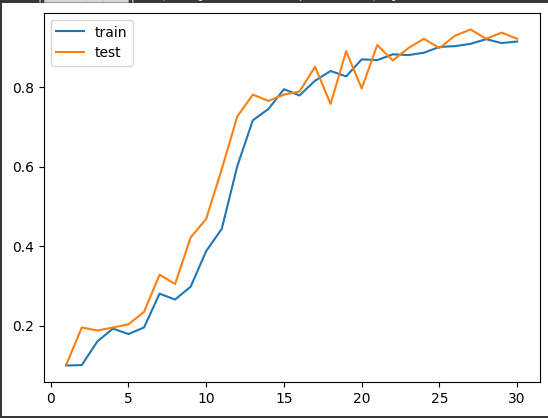
\includegraphics[width=0.8\textwidth]{images/res1.png}
\caption{}
\label{fig:img1}
\end{figure}

На рисунке ~\ref{fig:img2} приведен график точности модели LeNet с оптимизатором Adadelta и скоростью обучения 0.1.

\begin{figure}[H]
\centering
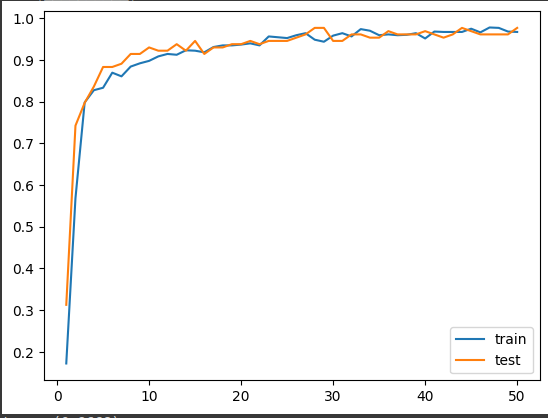
\includegraphics[width=0.8\textwidth]{images/res2.png}
\caption{}
\label{fig:img2}
\end{figure}

На рисунке ~\ref{fig:img3} приведен график точности модели LeNet с оптимизатором NAG и скоростью обучения 0.001.

\begin{figure}[H]
\centering
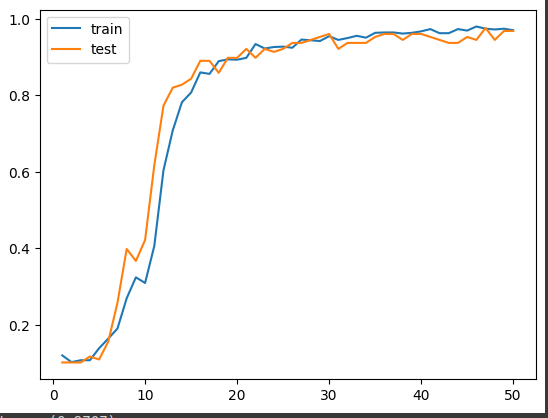
\includegraphics[width=0.8\textwidth]{images/res3.png}
\caption{}
\label{fig:img3}
\end{figure}

На рисунке ~\ref{fig:img3} приведен график точности модели LeNet с оптимизатором Adam и скоростью обучения 0.001.

\begin{figure}[H]
\centering
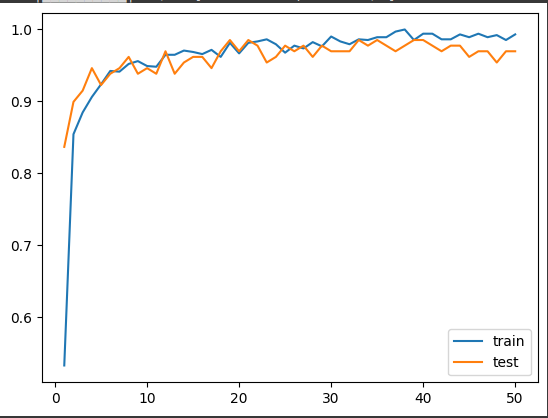
\includegraphics[width=0.8\textwidth]{images/res4.png}
\caption{}
\label{fig:img4}
\end{figure}

На рисунке ~\ref{fig:img5} приведен график точности модели MiniVGG с оптимизатором SGD и скоростью обучения 0.01.

\begin{figure}[H]
\centering
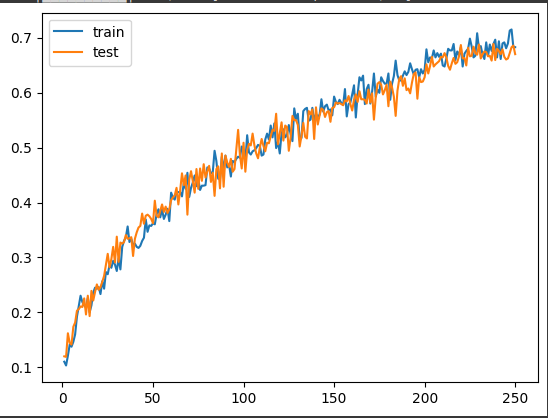
\includegraphics[width=0.8\textwidth]{images/res5.png}
\caption{}
\label{fig:img5}
\end{figure}

На рисунке ~\ref{fig:img6} приведен график точности модели MiniVGG с оптимизатором Adadelta и скоростью обучения 0.1.

\begin{figure}[H]
\centering
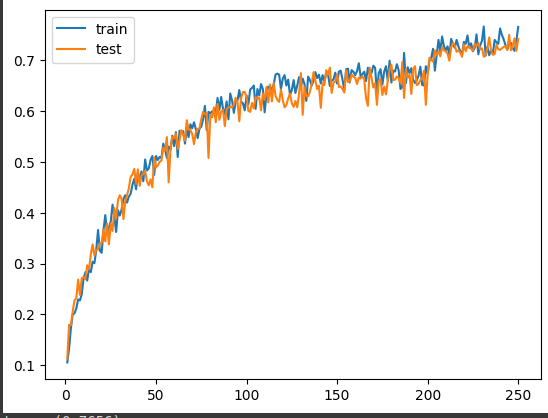
\includegraphics[width=0.8\textwidth]{images/res6.png}
\caption{}
\label{fig:img6}
\end{figure}

На рисунке ~\ref{fig:img7} приведен график точности модели MiniVGG с оптимизатором NAG и скоростью обучения 0.001.

\begin{figure}[H]
\centering
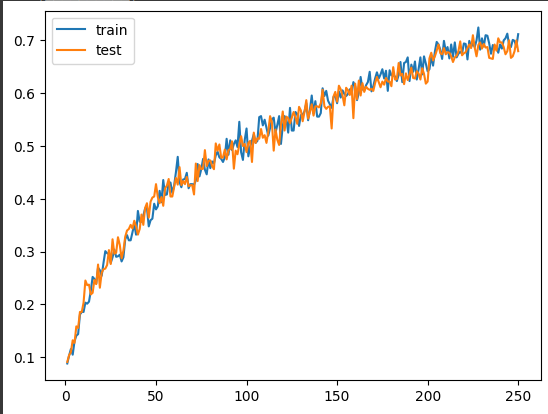
\includegraphics[width=0.8\textwidth]{images/res7.png}
\caption{}
\label{fig:img7}
\end{figure}

На рисунке ~\ref{fig:img8} приведен график точности модели MiniVGG с оптимизатором Adam и скоростью обучения 0.0001.

\begin{figure}[H]
\centering
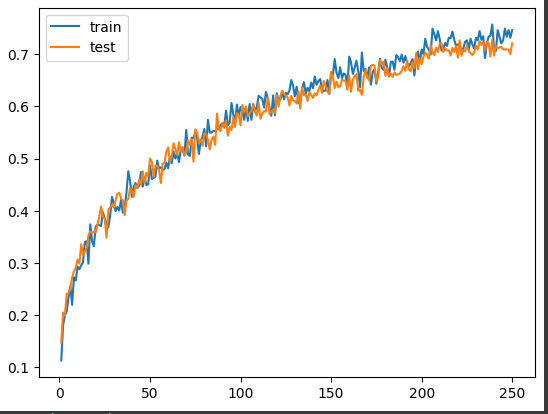
\includegraphics[width=0.8\textwidth]{images/res8.png}
\caption{}
\label{fig:img8}
\end{figure}


На рисунке ~\ref{fig:img9} приведен график точности модели ResNet с оптимизатором SGD и скоростью обучения 0.0015.

\begin{figure}[H]
\centering
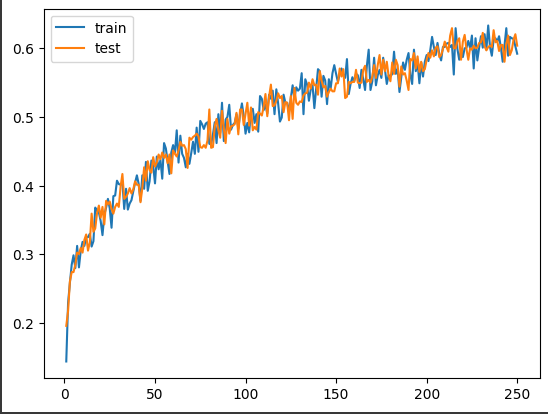
\includegraphics[width=0.8\textwidth]{images/res9.png}
\caption{}
\label{fig:img9}
\end{figure}


На рисунке ~\ref{fig:img10} приведен график точности модели ResNet с оптимизатором Adadelta и скоростью обучения 0.15.

\begin{figure}[H]
\centering
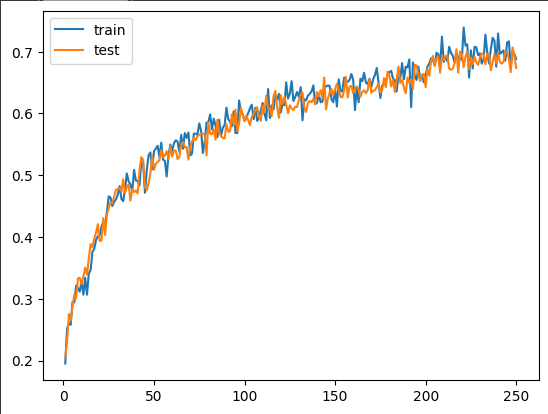
\includegraphics[width=0.8\textwidth]{images/res10.png}
\caption{}
\label{fig:img10}
\end{figure}

На рисунке ~\ref{fig:img11} приведен график точности модели ResNet с оптимизатором NAG и скоростью обучения 0.00015.

\begin{figure}[H]
\centering
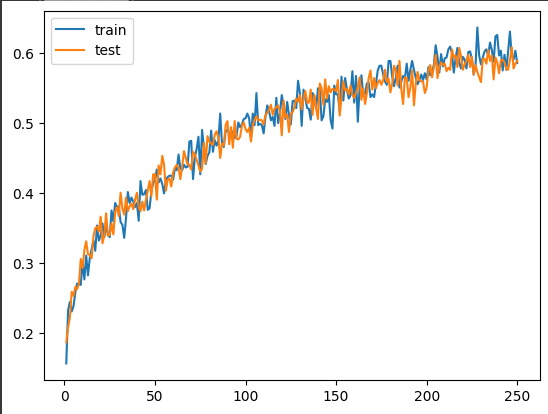
\includegraphics[width=0.8\textwidth]{images/res11.png}
\caption{}
\label{fig:img11}
\end{figure}


На рисунке ~\ref{fig:img12} приведен график точности модели ResNet с оптимизатором Adam и скоростью обучения 0.00015.

\begin{figure}[H]
\centering
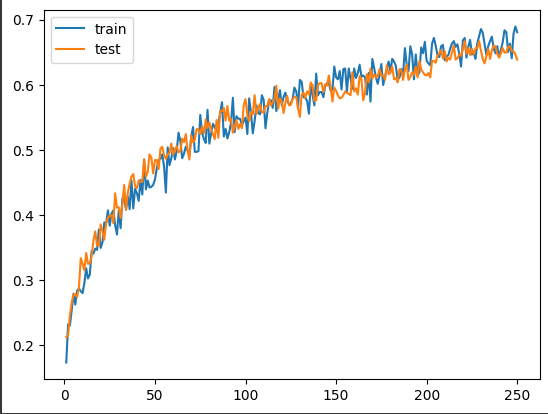
\includegraphics[width=0.8\textwidth]{images/res12.png}
\caption{}
\label{fig:img12}
\end{figure}

В таблице ~\ref{tab1:LeNet} приведена вариация гиперпараметров для модели LeNet.

\begin{table}[h]
\centering
\caption{}
\label{tab1:LeNet}
\begin{tabular}{|c|c|c|c|}
  \hline
  Оптимизатор & Кол-во эпох  & Скорость обучения & Точность \\
  \hline
  SGD & 30 & 0.0055 & 0.9150 \\
  \hline
  Adadelta & 50 & 0.1 & 0.9668 \\
  \hline
  NAG & 50 & 0.001 & 0.9707 \\
  \hline
  Adam & 50 & 0.001 & 0.9922 \\
  \hline
\end{tabular}
\end{table}

В таблице ~\ref{tab2:VGG} приведена вариация гиперпараметров для модели MiniVGG.

\begin{table}[h]
\centering
\caption{}
\label{tab2:VGG}
\begin{tabular}{|c|c|c|c|c|}
  \hline
  Оптимизатор & Кол-во эпох  & Скорость обучения & Dropout & Точность \\
  \hline
  SGD & 250 & 0.01 & 0.5 & 0.6826 \\
  \hline
  Adadelta & 250 & 0.1 & 0.5 & 0.7656 \\
  \hline
  NAG & 250 & 0.001 & 0.5 & 0.7119 \\
  \hline
  Adam & 250 & 0.0001 & 0.5 & 0.7461 \\
  \hline
\end{tabular}
\end{table}

В таблице ~\ref{tab3:ResNet} приведена вариация гиперпараметров для модели ResNet.

\begin{table}[h]
\centering
\caption{}
\label{tab3:ResNet}
\begin{tabular}{|c|c|c|c|c|}
  \hline
  Оптимизатор & Кол-во эпох  & Скорость обучения & Dropout & Точность \\
  \hline
  SGD & 250 & 0.0015 & 0.5 & 0.5918 \\
  \hline
  Adadelta & 250 & 0.15 & 0.5 & 0.6807 \\
  \hline
  NAG & 250 & 0.00015 & 0.5 & 0.5859 \\
  \hline
  Adam & 250 & 0.00015 & 0.5 & 0.6885 \\
  \hline
\end{tabular}
\end{table}



\section{Выводы}
В рамках данной лабораторной работы с помощью популярного фреймворка PyTorch были реализованы следующие архитектуры сверточных нейронных сетей: LeNet, MiniVGG, ResNet. Среди экспериментов с LeNet лучшей оказалась модель с оптимизатором Adam и скоростью обучения 0.001. Среди экспериментов с MiniVGG лучшей оказалась модель с оптимизатором Adadelta и скоростью обучения 0.1. Среди экспериментов с ResNet лучшей оказалась модель с оптимизатором Adam и скоростью обучения 0.15.
\end{document}